\section{Location calculation techniques} 
\label{sec:techniques} 
 
 
This section's focus is on the available means of obtaining distance measurements from a mobile target to a beacon. Figure \ref{fig:BeSP} displays a representation of the beacon-smartphone interaction. Whenever a location calculation is requested, the collection of data from nearby reference points is mandatory. In indoor location systems, these reference points are provided by beacons deployed in the location environment. The type of information collected, that is afterwards translated into distance, can be of several different types. The following section will target the different means of obtaining distances, as well as how to calculate a location from them.  

\begin{figure}[H] 
\centering 
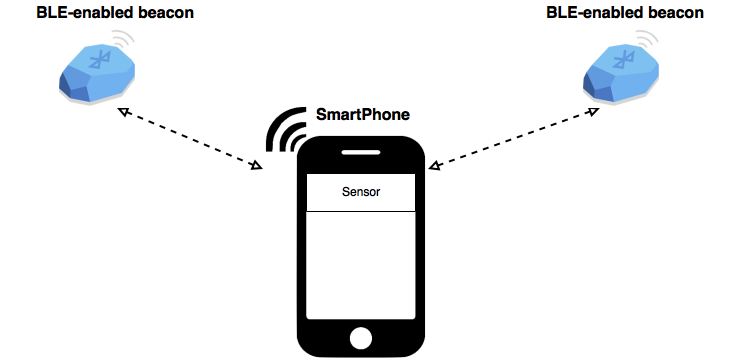
\includegraphics[width=0.65\linewidth]{2.Chapter/Beacon+SP.png} 
\caption[Beacon and Smartphone interaction]{Beacon and Smartphone interaction} 
\label{fig:BeSP} 
\end{figure} 

\subsection{Proximity Detection} 
\label{subsec:prox} 
 
 
Proximity detection is one of the simplest position techniques to implement since its objective isn't to provide a precise position of the target but a symbolic relative location information\cite{reviewtechniques}. The target's position is obtained through the \ac{CoO} method which relies on a grid of antennas/beacon with a well-known position. When applying this method, if only one beacon is detected by the mobile target then the position provided is equal to the position of the beacon. If more than one beacons are detected by the target, it considers that its position is equal to the position of beacon with the strongest associated signal. In order to apply room-based accuracy, the minimum requirement would be to place a beacon in each existent room. This method can be applied with a better accuracy in mind and doing so, it depends only on the deployed beacon density. This technique is often implemented in systems running \ac{IR} , \ac{RFID} and Bluetooth. 
 
 

\subsection{Triangulation} 
\label{subsec:tri} 
 

 
The Triangulation techniques make use of the geometric properties of triangles to determine the location of a mobile target. It can be of two types: lateration, which estimates a target's position by measuring its distance to multiple reference points, and angulation, which obtains the target's position by computing angles relative to multiple reference points. The metrics used for location calculation with either of the types, will now be presented. 



\subsubsection{Time of Arrival (ToA) } 
\label{subsubsec:toa} 
 
 
\ac{ToA}-based systems rely on accurate clock synchronisation and signal message sent from a mobile target to several receiving beacons \cite{locationtechniques}. The distance that is to be used in the calculation of the target's position is proportional to the propagation time. The message sent from the mobile target is timestamped with its departure time allowing for the receiving beacons to obtain their distance to the target through the transmission time and the associated signal propagation speed. 
One of the consequences of requiring precise knowledge of transmission start times is that every single device, beacon and mobile target, need to be accurately synchronised with a precise time source which causes this technique to be the most accurate one in indoor environments since it's capable of filtering multi-path effects. On the other hand, the disadvantages of using this technique is the synchronisation requirements and the additional information that needs to be contained in the sent messages, i.e. timestamps.  
 
 
 
 
\subsubsection{Time Difference of Arrival (TDoA) } 
\label{subsubsec:tdoa} 
 
 
\ac{TDoA} systems attempt to determine the relative position of a mobile target by examining the differences in time at which the signal arrives at multiple beacons\cite{TDoA}. This technique doesn't require clock synchronisation with the sender as there is no need for timestamps to obtain its location, making this requirement only present on the receivers. The location is obtained from a transmission with unknown starting time that is received in multiple synchronised receivers which produces multiple \ac{TDoA} measurements. Each difference in arrival times produces a \ac{TDoA} and consequently a hyperbolic curve on which the target is located. Each intersection of multiple hyperbolic curves represents a possible location of the target, requiring two or more measurements in order to obtain the location on a two dimensional plane. 
 
 
 
 
\subsubsection{Roundtrip Time of Flight (RToF)} 
\label{subsubsec:rtfo} 
 
 
This technique obtains distances by measuring the time-of-flight of the signal pulse traveling from the transmitter to the receiver ( measuring unit) and back\cite{rtfo}. This solution solves some of the synchronisation issues presented by \ac{ToA} since one of the two nodes records the transmission and arrival times, with the conversion from time to distance being equal to the one applied with \ac{ToA}. The mechanism of obtaining a time reading is similar to that of a radar, i.e. a signal is sent to the receiving node which replies back to the transmitter. When the response signal is received the roundtrip time is obtained. One issue presented by using this technique is the incapability of knowing the time delay on the receiver between receiving the first signal and sending the response. This unknown delay can be ignored in medium to long-ranged systems, if its value is relatively small when compared to the transmission time. In short-ranged system this situation can't be applied and therefore this technique isn't suited to be applied. 
 
 
 
 
\subsubsection{ \ac{RSSI}} 
\label{subsubsec:rssi} 
 
 
Received Signal Strength Information (RSSI) is a non-linear signal strength indicator based on signal attenuation that is only usable with radio signals. The conversion of this value to distance is often achieved through estimates of signal path loss due to propagation, although this approach doesn't hold in scenarios where severe multipath effects and shadowing are present. 
 
 
A technique that is often used with \ac{RSSI} is the fingerprint method which is the process of computing the location of a user by matching its location-dependent signal characteristics to an existing fingerprint database. This method doesn't require any additional hardware on the mobile device or the beacons as well as no time synchronisation. This process is divided in two stages: an offline and an online phase. In the offline stage, also called calibration phase, the maps for the fingerprint are set up either empirically in measurement operations or computed analytically through a signal propagation model. For the first option, multiple positions are defined on the map. On each of this positions a mobile user captures the signal strengths received from each of the existent beacons. An example of this method's data collection setup can be seen on Figure \ref{fig:fp}. With the fingerprint concluded, begins the online phase, where mobile users are already capable of being tracked. In order to obtain a user's position, it must measure the existent signal properties, which are then compared with the fingerprint database so that a close as possible match can be found. Position matching can be achieved through pattern recognition techniques such as K-nearest-neighbours (KNN), support vector machines (SVM), among others. 
This approach has the drawbacks of being labour intensive and time consuming on the offline phase and the difficulty to maintain and update the fingerprint database in order to be in accordance with the current environment. The second drawback is caused by \ac{RSSI}'s sensibility to changes in the environment such as dynamic factors (people and doors), diffraction and reflection.  
 
\begin{figure}[H] 
\centering 
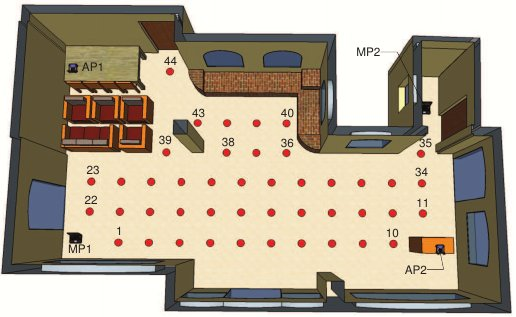
\includegraphics[width=0.5\linewidth]{2.Chapter/fp.jpg} 
\caption[Fingerprint example with data collection positions (Ref \cite{fingerprint}) ]{ Fingerprint example with data collection positions (Ref \cite{fingerprint}) } 
\label{fig:fp} 
\end{figure} 
 
 
\subsubsection{Angle of Arrival (AoA) } 
\label{subsubsec:aoa} 
 
 
The \ac{AoA} technique finds the location of the target by intersecting several pairs of angle direction lines. Each of these lines is part of the circular radius around a beacon which leads to the mobile target. This technique requires only two beacons for two dimensional and three for three dimensional position estimation, with any extra beacon leading to an increase in accuracy while not requiring any time synchronisation\cite{anglearrival}.  
This technique has two drawbacks: Increased implementation cost, since antennas capable of measuring angles are costly; Rapid accuracy degradation, i.e. the accuracy is heavily affected by the distance between user and beacon. This technique is capable of sub-meter accuracy although these types of systems are often limited by shadowing, multi-path reflections arriving from misleading directions or by the directivity of the measuring aperture.  
One example which attempted to tackle \ac{AoA}'s drawbacks was ArrayTrack \cite{arraytrack} which presented a multipath suppression algorithm capable of removing reflection paths, performance improvements in low density scenarios and parallel processing allowing for faster location estimations. This system was capable of achieving a median accuracy of 23 cm while utilising custom made access points with 16 antennas. Although successful, the hardware complexity remained an issue making this system impractical. 
 
 
\subsection{Dead Reckoning} 
\label{subsec:dr} 
 
 
\ac{DR} is the process of estimating the target's current position through the last determined position incremented by known or estimated speeds over elapsed time. This technique has the advantage of providing autonomous positioning capacities. \ac{DR} biggest drawback is that the inaccuracy of the process is cumulative, once the deviation in the position estimation grows with time. This issue can be aggravated by disruptive motion such as sidestepping, back-stepping or sharp turns which produce scaling errors leading to bigger accuracy errors. Due to \ac{DR}'s issues it's often accompanied by another technology in order to correct the inertial drift. A common practice is the usage of GPS, which doesn't function in indoor environments, leading to the implementation of many different combinations, in an attempt to tackle this issue. Fischer et al. \cite{dr1} made use of Ultrasound beacons as landmarks to provide better accuracy and less heading errors. In their work they stated the existence of two types of errors: heading errors, which are relative to the direction in which the user is heading, and distance errors. The work was targeted for rescue team first responders and required the users to drop ultrasonic beacons as they advanced through the building. 